\documentclass{article}
\usepackage{amsmath}
\usepackage{amssymb}
\usepackage{tikz}
\usepackage{geometry}
\geometry{a4paper, margin=1in}

\begin{document}

\section*{Derivation of the Rotation Matrix (Fig. 1)}

A scalar matrix (of square type) that is used to represent a rotational frame around the coordinate axes, commonly used in Euler angles and then Cardan angles.

\vspace{0.5em}

$\Rightarrow$ The rotation around x-axis is in the Z-convention (i.e., the angle of the rotation is with respect to the positive direction of Z-axis).

\vspace{0.5em}

Let $\vec{V}$ be a vector in an $R^3$ vector-space:

\begin{equation*}
\vec{V} = \begin{pmatrix}
\|\vec{V}\| \cdot \cos(\Phi_{(\vec{V}, \vec{V}_x)}) \\
\|\vec{V}_{yz}\| \cdot \cos\left(\frac{\pi}{2} - \Phi_{(\vec{V}_{yz}, \vec{V}_z)}\right) \\
\|\vec{V}_{yz}\| \cdot \cos(\Phi_{(\vec{V}_{yz}, \vec{V}_z)})
\end{pmatrix}
\end{equation*}

\vspace{0.5em}

Then, using the Euclidean Geometry, one could deduce the newly rotated vector $\vec{V}^{'}$ around the X-axis by 
angle of $\hat{\Phi_{R}}$ with the positive direction of Z-axis in the YZ Vectorspace:

\begin{equation*}
\vec{V}^{'} = \begin{pmatrix}
\|\vec{V}\| \cdot \cos(\Phi_{(\vec{V}, \vec{V}_x)}) \\
\|\vec{V}_{yz}\| \cdot \cos\left(\frac{\pi}{2} - (\Phi_{(\vec{V}_{yz}, \vec{V}_z)} \pm \Phi_{R_x})\right) \\
\|\vec{V}_{yz}\| \cdot \cos(\Phi_{(\vec{V}_{yz}, \vec{V}_z)} \pm \Phi_{R_x})
\end{pmatrix}
\end{equation*}
is the vectorial structure for representing angular motion around the x-axis using the Z-convention.

\vspace{0.5em}


\begin{align*}
\because\quad
& \cos(\phi \pm \alpha) = \cos(\phi)\cos(\alpha) \mp \sin(\phi)\sin(\alpha) \\
& , \cos (\frac{\pi}{2} - \theta) = \sin(\theta) \\
& , \sin(\phi \pm \alpha) = \sin(\phi)\cos(\alpha) \pm \cos(\phi)\sin(\alpha) \\
& , (\text{Matrix}_{m \times n} \times \text{Matrix}_{n \times 1}) = \text{Matrix}_{m \times 1} \\
& , m = n = 3
\end{align*}

\vspace{0.5em}

Let $\|\vec{V}_{yz}\| = 1$; as $\vec{V}_{yz}$ is a unit vector in an R(2) vectorspace.

\vspace{0.5em}

$\therefore$ The rotated vector could be rewritten as a function of the rotational angle
    by evaluating the addition trigonometric identity: 

\begin{equation*}
\vec{V}^{'} = \begin{pmatrix}
\cos(\Phi_{(\vec{V}, \vec{V}_x)}) \\
\sin(\Phi_{(\vec{V}_{yz}, \vec{V}_z)})\cos(\Phi_{R}) \pm \cos(\Phi_{(\vec{V}_{yz}, \vec{V}_z)})
                \sin(\Phi_{R}) \\
\cos(\Phi_{(\vec{V}_{yz}, \vec{V}_z)})\cos(\Phi_{R}) \mp \sin(\Phi_{(\vec{V}_{yz}, \vec{V}_z)})
            \sin(\Phi_{R}) \\
\end{pmatrix}
\end{equation*}

\vspace{0.5em}

$\therefore$ The rotated vector in terms of the trigonometric identity could be rewritten using 
matrix algebra into a matrix product of a rotation matrix and the vector column matrix:

\[ 
\vec{V}^{'}: (\pm \hat{\Phi_R}) = R \times \vec{V} \\
            = \begin{pmatrix}
                1 & 0 & 0 \\
                0 & \cos(\Phi_{R}) & \pm \sin(\Phi_{R}) \\
                0 & \mp \sin(\Phi_R) & \cos(\Phi_{R})
              \end{pmatrix} 
              \times
              \begin{pmatrix}
               \cos(\Phi_{(\vec{V}, \vec{V}_x)}) \\
               \sin(\Phi_{(\vec{V}_{yz}, \vec{V}_z)}) \\
               \cos(\Phi_{(\vec{V}_{yz}, \vec{V}_z)})
              \end{pmatrix}
\]

\newpage

% --- Content for Image 2: WhatsAppImage2025-11-08at10.17.38_abe7f755.jpg ---
\section*{Rotation Matrix Construction (Image 2)}

To construct a rotation around the x-axis (J-convention), one could construct a rotation matrix. The cross product and vector $\vec{V}_0$ will attain a new rotated vector $\vec{V}_1$ by angle $\Phi_R$:

\begin{equation*}
\vec{V}_1 = \begin{pmatrix}
1 & 0 & 0 \\
0 & \cos(\Phi_R) & \sin(\Phi_R) \\
0 & -\sin(\Phi_R) & \cos(\Phi_R)
\end{pmatrix}
\begin{pmatrix}
V_{x0} \\
V_{y0} \\
V_{z0}
\end{pmatrix}
\end{equation*}

\textbf{NB:} The product multiplies a $3 \times 3$ matrix by a column vector. The result is a column vector representing the rotated vector.

\vspace{0.5em}

\begin{align*}
\therefore\ (\hat{\Phi}_R \text{ is } +\text{ve}) &\Rightarrow R_{yz} = \sin(\hat{\Phi}_R) \\
(\hat{\Phi}_R \text{ is } -\text{ve}) &\Rightarrow R_{yz} = -\sin(\hat{\Phi}_R)
\end{align*}

\vspace{0.5em}

$R_{yz} = \sin(\Phi_R)$

\vspace{0.5em}

$\hat{\Phi}_R = +(- \hat{\Phi}_R)$

\vspace{0.5em}

We could rewrite the equation as:
\begin{equation*}
\vec{V}_1 = \begin{pmatrix}
1 & 0 & 0 \\
0 & \cos(\Phi_R) & \sin(\Phi_R) \\
0 & -\sin(\Phi_R) & \cos(\Phi_R)
\end{pmatrix}
\begin{pmatrix}
V_{x0} \\
V_{y0} \\
V_{z0}
\end{pmatrix}
\end{equation*}

\textbf{NB:} The $(+)$ and $(-)$ signs are bound to the angle of rotation $\Phi_R$; if $\Phi_R$ is +ve then the $R_{yz}$ component will be +ve, if $\Phi_R$ is -ve then $R_{yz}$ will be negative; $R_{zy}$ component is +ve when the angle is -ve.

\vspace{0.5em}

\begin{align*}
\sin(-\Phi_R) &= -\sin(\Phi_R) \\
\cos(-\Phi_R) &= \cos(\Phi_R)
\end{align*}

\textbf{NB:} The normal formula assumes the angle is +ve; even for -ve angles $\sin(-\Phi_R) = -\sin(\Phi_R)$.

\newpage

% --- Content for Image 3: WhatsAppImage2025-11-08at10.17.37_3f101545.jpg ---
\section*{Remarks on Vector Rotation (Image 3)}

\# Remarks:

\vspace{0.5em}
\begin{itemize}
\item To rotate a vector in the $\mathbb{R}^3$ vector space about the $y$-axis, the angles of projection of that vector component in the $xy$ plane could be adjusted.
\end{itemize}

\vspace{0.5em}
(1) Projection onto a surface area:

\begin{center}
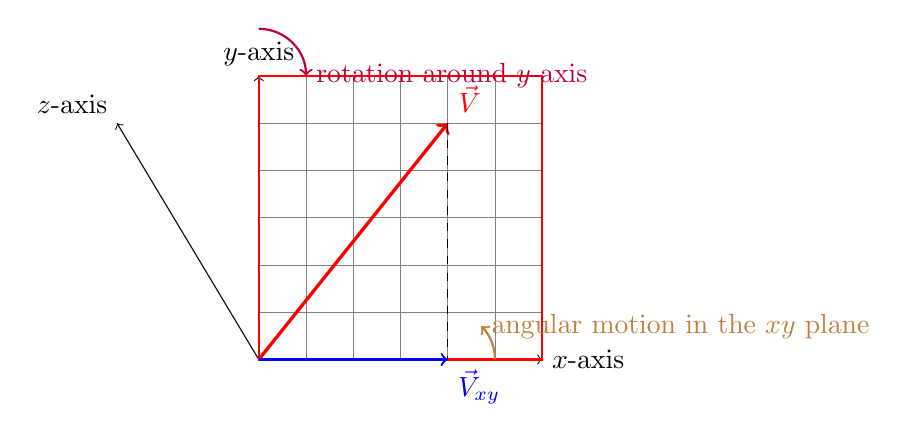
\begin{tikzpicture}[scale=1.2]
    % Define coordinates
    \coordinate (O) at (0,0);
    \coordinate (X) at (3,0);
    \coordinate (Y) at (0,3);
    \coordinate (Z) at (-1.5, 2.5);
    \coordinate (V) at (2, 2.5);

    % Axes
    \draw[->] (O) -- (X) node[right] {$x$-axis};
    \draw[->] (O) -- (Y) node[above] {$y$-axis};
    \draw[->] (O) -- (Z) node[above left] {$z$-axis};

    % Projection plane (xy-plane) grid
    \draw[gray, dashed] (3,0) -- (3,3) -- (0,3);
    \foreach \x in {0.5, 1.0, 1.5, 2.0, 2.5}
        \draw[gray, very thin] (\x, 0) -- (\x, 3);
    \foreach \y in {0.5, 1.0, 1.5, 2.0, 2.5}
        \draw[gray, very thin] (0, \y) -- (3, \y);
    \draw[red, thick] (0,0) rectangle (3,3);

    % Vector V
    \draw[->, very thick, red] (O) -- (V) node[above right] {$\vec{V}$};

    % Projection of V onto xy-plane (V_xy)
    \coordinate (Vxy) at (2, 0);
    \draw[dashed] (V) -- (Vxy);
    \draw[->, thick, blue] (O) -- (Vxy) node[below right] {$\vec{V}_{xy}$};

    % Rotation around y-axis
    \draw[->, thick, purple] (0, 3.5) arc (90:0:0.5) node[right] {rotation around $y$-axis};

    % Angular motion in xy-plane (rotation around z-axis)
    \draw[->, thick, brown] (2.5, 0) arc (0:45:0.5) node[right] {angular motion in the $xy$ plane};
\end{tikzpicture}
\end{center}

\begin{equation*}
\vec{V}_y = \begin{pmatrix}
\|\vec{V}_0\| \cdot \cos(\Phi_{\vec{V}_0}) \\
\frac{\partial}{\partial \vec{V}_y} \cdot \cos\left(\frac{\pi}{2} - (\Phi_{\vec{V}_0} \pm \Phi_{R_z})\right) \\
\frac{\partial}{\partial \vec{V}_z} \cdot \cos(\Phi_{\vec{V}_0} \pm \Phi_{R_z})
\end{pmatrix}
\end{equation*}

\vspace{0.5em}
\begin{itemize}
\item To rotate a vector in the $\mathbb{R}^3$ vector space about the $x$-axis, the angles of projection of that vector component in the $yz$ plane could be adjusted.
\end{itemize}

\begin{center}
\begin{tikzpicture}[scale=1.2]
    % Define coordinates
    \coordinate (O) at (0,0);
    \coordinate (X) at (3,0);
    \coordinate (Y) at (-1.5, 2.5);
    \coordinate (Z) at (0,3);
    \coordinate (V) at (2, 2.5);

    % Axes
    \draw[->] (O) -- (X) node[right] {$x$-axis};
    \draw[->] (O) -- (Y) node[above left] {$y$-axis};
    \draw[->] (O) -- (Z) node[above] {$z$-axis};

    % (Simplified) Projection plane (yz-plane)
    \draw[gray, dashed] (Y) -- ++(0, -2.5) -- ++(1.5, 0) -- ++(0, 2.5);
    \draw[red, thick] (O) -- (Y) -- ++(0, 3) -- (Z) -- cycle;

    % Vector V
    \draw[->, very thick, red] (O) -- (V) node[above right] {$\vec{V}$};

    % Rotation around x-axis
    \draw[->, thick, purple] (3.5, 0) arc (0:-90:0.5) node[below] {rotation around $x$-axis};

    % Angular motion in yz-plane
    \draw[->, thick, brown] (0, 2.5) arc (90:135:0.5) node[left] {angular motion in the $yz$ plane};
\end{tikzpicture}
\end{center}

\begin{equation*}
\vec{V}_x = \begin{pmatrix}
\|\vec{V}_0\| \cdot \cos(\Phi_{\vec{V}_0}) \\
\frac{\partial}{\partial \vec{V}_y} \cdot \cos(\Phi_{\vec{V}_0} \pm \Phi_{R_x}) \\
\frac{\partial}{\partial \vec{V}_z} \cdot \cos(\Phi_{\vec{V}_0} \pm \Phi_{R_x})
\end{pmatrix}
\end{equation*}

\vspace{0.5em}
Let $\vec{V}_0$ be zero, determining the initial position of motion (kinematics).

\vspace{0.5em}
$\therefore (\vec{V}_0, \dots, \vec{V}_n)$ sequence could be obtained in a time interval defining a differential equation of displacement (angular) $\Rightarrow$ velocity.

\newpage

% --- Content for Image 4: WhatsAppImage2025-11-08at10.17.37_163fcbc9.jpg ---
\section*{Rotation about $\vec{V}_y$ axis (Image 4)}

To rotate a vector in $\mathbb{R}^3$ vector space about the $\vec{V}_y$ axis, adjust the angles of projection of that vector component in the $xy$ plane.

\vspace{0.5em}
(1) Projection onto a surface area:

\begin{center}
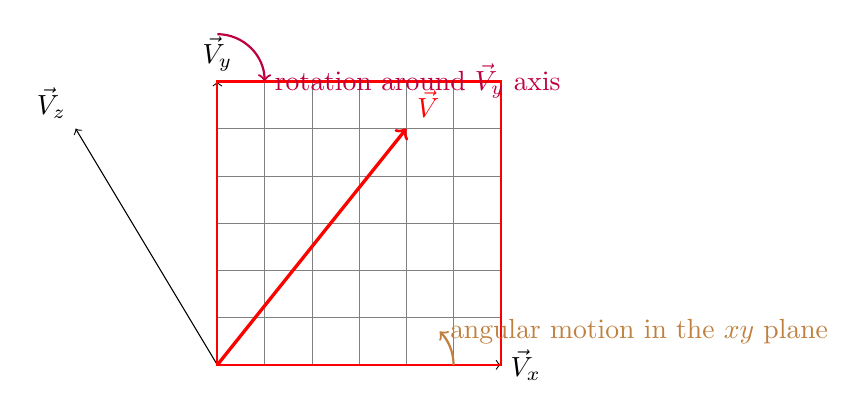
\begin{tikzpicture}[scale=1.2]
    % Define coordinates
    \coordinate (O) at (0,0);
    \coordinate (Vx) at (3,0);
    \coordinate (Vy) at (0,3);
    \coordinate (Vz) at (-1.5, 2.5);
    \coordinate (V) at (2, 2.5);

    % Axes
    \draw[->] (O) -- (Vx) node[right] {$\vec{V}_x$};
    \draw[->] (O) -- (Vy) node[above] {$\vec{V}_y$};
    \draw[->] (O) -- (Vz) node[above left] {$\vec{V}_z$};

    % Projection plane (xy-plane) grid
    \draw[gray, dashed] (3,0) -- (3,3) -- (0,3);
    \foreach \x in {0.5, 1.0, 1.5, 2.0, 2.5}
        \draw[gray, very thin] (\x, 0) -- (\x, 3);
    \foreach \y in {0.5, 1.0, 1.5, 2.0, 2.5}
        \draw[gray, very thin] (0, \y) -- (3, \y);
    \draw[red, thick] (0,0) rectangle (3,3);

    % Vector V
    \draw[->, very thick, red] (O) -- (V) node[above right] {$\vec{V}$};

    % Rotation around Vy-axis
    \draw[->, thick, purple] (0, 3.5) arc (90:0:0.5) node[right] {rotation around $\vec{V}_y$ axis};

    % Angular motion in xy-plane
    \draw[->, thick, brown] (2.5, 0) arc (0:45:0.5) node[right] {angular motion in the $xy$ plane};
\end{tikzpicture}
\end{center}

\begin{equation*}
\vec{V}_0 = \begin{pmatrix}
\|\vec{V}_0\| \cdot \cos(\Phi_{\vec{V}_0}) \\
\|\vec{V}_0\| \cdot \cos\left(\frac{\pi}{2} - (\Phi_{\vec{V}_0} \pm \Phi_{R_y})\right) \\
\|\vec{V}_0\| \cdot \cos(\Phi_{\vec{V}_0} \pm \Phi_{R_y})
\end{pmatrix}
\end{equation*}
... angle of rotation of motion around the $\vec{V}_y$ axis.

\newpage

% --- Content for Image 5: WhatsAppImage2025-11-08at10.17.34_6bacdd29.jpg ---
\section*{Co-functions and Projection Vector (Image 5)}

\textbf{NB:} Sine and cosine are co-functions.

\begin{align*}
\sin\left(\frac{\pi}{2} - \Phi\right) &= \cos(\Phi) \\
\cos\left(\frac{\pi}{2} - \Phi\right) &= \sin(\Phi)
\end{align*}

\vspace{0.5em}

Therefore equation $\vec{V}_{0y}$ of the linear projection vector $(\text{proj}_{\vec{V}_y}(\vec{V}_0))$ could be rewritten as:

\begin{equation*}
\text{proj}_{\vec{V}_y}(\vec{V}_0) = \begin{pmatrix}
\|\vec{V}_0\| \cdot \cos\left(\frac{\pi}{2} - \Phi\right) \\
\|\vec{V}_0\| \cdot \cos(\Phi)
\end{pmatrix}
\end{equation*}

\begin{equation*}
= \begin{pmatrix}
\|\vec{V}_0\| \cdot \sin(\Phi) \\
\|\vec{V}_0\| \cdot \cos(\Phi)
\end{pmatrix}
\end{equation*}

\newpage

% --- Content for Image 6: WhatsAppImage2025-11-08at10.17.34_41a0d26b.jpg ---
\section*{Finding Projection Vectors on Axes (Image 6)}

Finding projection vectors of $\vec{V}_0$ on the vector space axes:

\vspace{0.5em}

$\Rightarrow \text{proj}_{\vec{V}_x}(\vec{V}_0)$: The vector that projects on $\vec{V}_x$ as a result of $\vec{V}_0$ is the same as the component $\vec{V}_x$ of the vector $\vec{V}_0$. $\text{proj}_{\vec{V}_x}(\vec{V}_0) \equiv \vec{V}_{0x}$ and can be calculated by examining the angle that $\vec{V}_0$ makes with the $\vec{V}_x$ unit vector.

\vspace{0.5em}

$\therefore \text{proj}_{\vec{V}_x}(\vec{V}_0) = \begin{pmatrix}
\|\vec{V}_0\| \cdot \cos(\Phi_{\vec{V}_0}) \\
0
\end{pmatrix} \cdot \begin{pmatrix}
\|\vec{V}_x\| \\
0
\end{pmatrix}$

\vspace{0.5em}

$\Phi_{\vec{V}_0}$ is the angle of projection of $\vec{V}_0$ on the $\vec{V}_x$ vector.

\vspace{0.5em}

$\Rightarrow \text{proj}_{\vec{V}_y}(\vec{V}_0)$: The vector that projects on $\vec{V}_y$ as a result of $\vec{V}_0$ is the same as the component $\vec{V}_y$ of the vector $\vec{V}_0$. $\text{proj}_{\vec{V}_y}(\vec{V}_0) \equiv \vec{V}_{0y}$ and can be calculated by examining the angle that $\vec{V}_0$ makes with the $\vec{V}_y$ unit vector and the direction of vector $\vec{V}_y$.

\vspace{0.5em}

$\therefore \text{proj}_{\vec{V}_y}(\vec{V}_0) = \begin{pmatrix}
0 \\
\|\vec{V}_0\| \cdot \sin(\Phi_{\vec{V}_0})
\end{pmatrix} \cdot \begin{pmatrix}
0 \\
\|\vec{V}_y\|
\end{pmatrix}$

\vspace{0.5em}

$\Phi_{\vec{V}_0}$ is the angle of projection of $\vec{V}_0$ on the $\vec{V}_x$ vector.

\vspace{0.5em}
$\Phi_{\vec{V}_0}'$ is the complementary angle.

\vspace{0.5em}

$\omega_{\vec{V}_0}$ is the angle of projection of $\vec{V}_0$ on $\vec{V}_y$.

\newpage

% --- Content for Image 7: WhatsAppImage2025-11-08at10.17.37_b6e1cda1.jpg ---
\section*{Projection Vector on $\vec{V}_y$ (Image 7)}

$\Rightarrow \text{proj}_{\vec{V}_y}(\vec{V}_0)$: is the projection vector on the $\vec{V}_y$ vector as a result of $\vec{V}_0$. 

\vspace{0.5em}
\textbf{NB:} $\cos(\hat{\Phi}_{\vec{V}_0, \vec{V}_y}) = \cos\left(\frac{\pi}{2} - \hat{\Phi}_{\vec{V}_0, \vec{V}_x}\right)$

\begin{equation*}
\text{proj}_{\vec{V}_y}(\vec{V}_0) = \begin{pmatrix}
0 \\
\|\vec{V}_0\| \cdot \cos(\Phi) \\
0
\end{pmatrix} \cdot \begin{pmatrix}
0 \\
\|\vec{V}_y\| \\
0
\end{pmatrix}
\end{equation*}

\vspace{0.5em}

$\hat{\Phi}_{\vec{V}_0, \vec{V}_y}$ is the angle of projection of $\vec{V}_0$; the resultant vector from $\vec{V}_x$ and $\vec{V}_y$ component vectors on the unit vector $\vec{V}_y$.

\vspace{0.5em}

It has a complementary angle:

\vspace{0.5em}

$\hat{\Phi}_{\vec{V}_0, \vec{V}_{xy}} \equiv \Phi$; the angle of projection of the vector $\vec{V}_0$ on the resultant vector $\vec{V}_{xy}$ from the $x$ and $y$ planes.

\vspace{0.5em}

$\hat{\Phi}_{\vec{V}_0, \vec{V}_z} = \frac{\pi}{2} - \hat{\Phi}_{\vec{V}_0, \vec{V}_{xy}}$

Therefore, the equation for $\vec{V}_0$ could be rewritten into this form:

\begin{equation*}
\text{proj}(\vec{V}_0) = \begin{pmatrix}
0 \\
\|\vec{V}_0\| \cdot \sin(\hat{\Phi}_{\vec{V}_0, \vec{V}_{xy}}) \\
0
\end{pmatrix} \cdot \begin{pmatrix}
0 \\
\|\vec{V}_0\| \cdot \|\vec{V}_y\| \\
0
\end{pmatrix}
\end{equation*}

\textbf{NB:} $\sin\left(\frac{\pi}{2} - \Phi\right) = \cos(\Phi)$

\newpage

% --- Content for Image 8: WhatsAppImage2025-11-08at10.17.33_85e2d0bd.jpg ---
\section*{Transformation among 3D axes (Image 8)}

Transformation among 3D axes:

\begin{center}
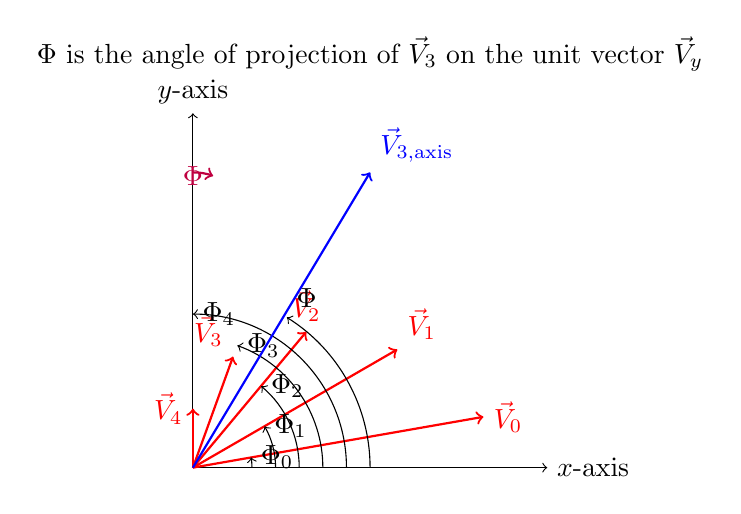
\begin{tikzpicture}[scale=1.5]
    % Define coordinates
    \coordinate (O) at (0,0);
    \coordinate (X) at (3,0);
    \coordinate (Y) at (0,3);
    \coordinate (Vthreeaxis) at (1.5, 2.5);

    % Axes
    \draw[->] (O) -- (X) node[right] {$x$-axis};
    \draw[->] (O) -- (Y) node[above] {$y$-axis};

    % Vectors (angles and lengths are placeholders)
    \draw[->, thick, red] (O) -- (2.46,0.43) node[right] {$\vec{V}_0$};
    \draw[->, thick, red] (O) -- (1.73,1.00) node[above right] {$\vec{V}_1$};
    \draw[->, thick, red] (O) -- (0.96,1.15) node[above] {$\vec{V}_2$};
    \draw[->, thick, red] (O) -- (0.34,0.94) node[above left] {$\vec{V}_3$};
    \draw[->, thick, red] (O) -- (0,0.5) node[left] {$\vec{V}_4$};

    % Angles (visual, not mathematically correct)
    \draw[->] (0.5, 0) arc (0:10:0.5) node[right] {$\Phi_0$};
    \draw[->] (0.7, 0) arc (0:30:0.7) node[right] {$\Phi_1$};
    \draw[->] (0.9, 0) arc (0:50:0.9) node[right] {$\Phi_2$};
    \draw[->] (1.1, 0) arc (0:70:1.1) node[right] {$\Phi_3$};
    \draw[->] (1.3, 0) arc (0:90:1.3) node[right] {$\Phi_4$};

    % V3,axis and angle Phi
    \draw[->, thick, blue] (O) -- (Vthreeaxis) node[above right] {$\vec{V}_{3,\text{axis}}$};
    \draw[->] (1.5, 0) arc (0:58:1.5) node[above right] {$\Phi$};

    % Angle Phi (projection on Vy)
    \draw[->, thick, purple] (0, 2.5) arc (90:70:0.5) node[left] {$\Phi$};
    \node at (1.5, 3.5) {$\Phi$ is the angle of projection of $\vec{V}_3$ on the unit vector $\vec{V}_y$};
\end{tikzpicture}
\end{center}

\vspace{0.5em}

Vector $\vec{V}_0$:
\begin{equation*}
\vec{V}_0 = \begin{pmatrix}
\|\vec{V}_0\| \cdot \cos(\hat{\Phi}_0) \\
\|\vec{V}_0\| \cdot \sin(\hat{\Phi}_0) \\
0
\end{pmatrix} = \begin{pmatrix}
\|\vec{V}_0\| \cdot \cos(\hat{\Phi}_0) \\
\|\vec{V}_0\| \cdot \sin(\hat{\Phi}_0) \\
0
\end{pmatrix}
\end{equation*}

\textbf{NB:} $(\hat{\Phi}_0)$ is the angle with the positive direction of x-axis.

\vspace{0.5em}

Complementary angle is $\Phi_0 = \frac{\pi}{2} - \hat{\Phi}_0$.

\vspace{0.5em}

\begin{equation*}
\vec{V}_0 = \begin{pmatrix}
0 \\
\|\vec{V}_0\| \cdot \cos(\hat{\Phi}_0) \\
0
\end{pmatrix}
+ 
\begin{pmatrix}
\|\vec{V}_0\| \cdot \sin(\hat{\Phi}_0) \\
0 \\
0
\end{pmatrix}
\end{equation*}

\vspace{0.5em}

$(\hat{\Phi})$ is the angle with the positive direction of $\vec{V}_x$. The resultant vector in the $xy$ plane is the angle of projection of $\vec{V}_0$ on vector $\vec{V}_{xy}$.

The complementary angle $\hat{\Phi}'_{xy} = \frac{\pi}{2} - \hat{\Phi}_{xy}$ is the angle of projection of vector $\vec{V}_{xy}$ on the unit vector $\vec{V}_y$.

\newpage

% --- Content for Image 9: WhatsAppImage2025-11-08at10.17.37_9a8ef274.jpg ---
\section*{Vector Construction and Projection (Image 9)}

Therefore, from equations 1, 2, and 3:

\vspace{0.5em}
\begin{enumerate}
\item Constructing vectors could be based on finding the projection vectors of the required vector on the unit vectors $\{\vec{V}_x, \vec{V}_y, \vec{V}_z\}$.
\end{enumerate}

\vspace{0.5em}

\begin{equation*}
\vec{V} = \begin{pmatrix}
\|\vec{V}\| \cdot \cos(\Phi_{\vec{V}}) \\
\|\vec{V}\| \cdot \cos(\Phi_{\vec{V}, \vec{V}_{xy}}) \\
\|\vec{V}\| \cdot \cos(\Phi_{\vec{V}, \vec{V}_z})
\end{pmatrix}
\end{equation*}

\begin{center}
\begin{tikzpicture}[scale=1.5]
    % Define coordinates
    \coordinate (O) at (0,0);
    \coordinate (X) at (3,0);
    \coordinate (Y) at (-1.5, 2.5);
    \coordinate (Z) at (0,3);
    \coordinate (V) at (2, 2.5);

    % Axes
    \draw[->] (O) -- (X) node[right] {$x$-axis};
    \draw[->] (O) -- (Y) node[above left] {$y$-axis};
    \draw[->] (O) -- (Z) node[above] {$z$-axis};

    % Unit Vectors
    \draw[->, dashed, blue] (O) -- (1, 0) node[below] {$\vec{V}_x$};
    \draw[->, dashed, blue] (O) -- (0, 1) node[left] {$\vec{V}_z$};
    \draw[->, dashed, blue] (O) -- (-0.5, 0.8) node[left] {$\vec{V}_y$};

    % Vector V
    \draw[->, very thick, red] (O) -- (V) node[above right] {$\vec{V}$};

    % Projection of V onto xy-plane (V_xy)
    \coordinate (Vxy) at (2, 0);
    \draw[dashed] (V) -- (Vxy);
    \draw[->, thick, green!60!black] (O) -- (Vxy) node[below right] {$\vec{V}_{xy}$};

    % Angle Phi_V
    \draw[->] (1.5, 0) arc (0:51:1.5) node[right] {$\Phi_{\vec{V}}$};
\end{tikzpicture}
\end{center}

Projection Component = Scalar

\vspace{0.5em}

$\frac{\text{directional vector}}{(\text{i.e., normalized vector})}$

\vspace{0.5em}

\textbf{NB:} $\vec{U} \cdot \vec{V} = \|\vec{U}\| \, \|\vec{V}\| \cos(\Phi_{\vec{U}, \vec{V}})$

\begin{center}
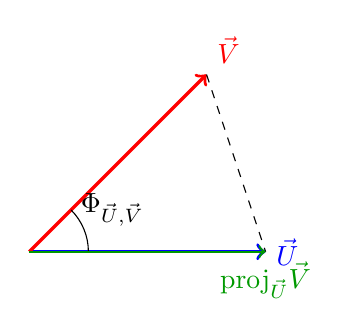
\begin{tikzpicture}[scale=1.5]
    % Define coordinates
    \coordinate (O) at (0,0);
    \coordinate (U) at (2,0);
    \coordinate (V) at (1.5, 1.5);

    % Vectors
    \draw[->, very thick, blue] (O) -- (U) node[right] {$\vec{U}$};
    \draw[->, very thick, red] (O) -- (V) node[above right] {$\vec{V}$};

    % Angle
    \draw (0.5, 0) arc (0:45:0.5) node[right] {$\Phi_{\vec{U}, \vec{V}}$};

    % Projection
    \coordinate (Vproj) at (2, 0);
    \draw[dashed] (V) -- (Vproj);
    \draw[->, thick, green!60!black] (O) -- (Vproj) node[below] {$\text{proj}_{\vec{U}}\vec{V}$};
\end{tikzpicture}
\end{center}

\begin{equation*}
= \|\vec{U}\| \cdot \|\vec{V}\| \cdot \cos(\Phi_{\vec{U}, \vec{V}})
\end{equation*}

\begin{equation*}
= \vec{U} \cdot \vec{V}
\end{equation*}

\vspace{0.5em}
Introducing a new scalar:
\begin{equation*}
\Rightarrow \text{proj}(\vec{V}) = \frac{\|\vec{U}\| \cdot \|\vec{V}\|}{\|\vec{U}\|}
\end{equation*}

\vspace{0.5em}
Finding its vector:
\begin{equation*}
\Rightarrow \text{proj}(\vec{V}) = \frac{\vec{U} \cdot \vec{V}}{\|\vec{U}\|} \cdot \vec{n}
\end{equation*}

\begin{equation*}
\Rightarrow \text{proj}(\vec{V}) = \frac{\vec{U} \cdot \vec{V}}{\|\vec{U}\|^2} \cdot \vec{U}
\end{equation*}

\newpage

% --- Content for Image 10: WhatsAppImage2025-11-08at10.17.37_038f1f1a.jpg ---
\section*{Projection Component (Image 10)}

\begin{equation*}
\text{proj}(\vec{V}) = \frac{\|\vec{U}\| \cdot \|\vec{V}\| \cdot \cos(\Phi_{\vec{U}, \vec{V}})}{\|\vec{U}\|}
\end{equation*}

\begin{equation*}
= \|\vec{V}\| \cdot \cos(\Phi_{\vec{U}, \vec{V}})
\end{equation*}

\begin{equation*}
= \frac{\vec{U} \cdot \vec{V}}{\|\vec{U}\|}
\end{equation*}

\vspace{0.5em}

$\text{proj}(\vec{V}) \cdot \vec{n}$

\vspace{0.5em}
$\frac{\text{Projection Component}}{(\text{Scalar})} \cdot \frac{\text{Projection direction}}{(\text{Vector unit})}$

\newpage

% --- Content for Image 11: WhatsAppImage2025-11-08at10.17.38_9fd30266.jpg ---
\section*{Lecture Notes on Rotation Matrices (Image 11)}

\begin{itemize}
\item Rotation matrices in $\mathbb{R}^3$ vector space are composed of 9 entries ($3 \times 3$); each row represents a linear algebraic equation of the new vector representing rotations of the vectorial components of the old vector ($\vec{V}_0$).
\item Each column houses the 3 coefficients of the rotational vectorial components ($V_{xx}$, $V_{xy}$, $V_{xz}$) for each vectorial component of the new vector.
\item To find the vectorial components ($V_{x1}$, $V_{y1}$, $V_{z1}$) of the new vector $\vec{V}_1$:
\end{itemize}

\begin{equation*}
V_{x1} = V_{xx} + V_{xy} + V_{xz} = 1
\end{equation*}

\begin{equation*}
V_{y1} = V_{yx} + V_{yy} + V_{yz} = \cos(\Phi_R) + \sin(\Phi_R)
\end{equation*}

\begin{equation*}
V_{z1} = V_{zx} + V_{zy} + V_{zz} = \cos(\Phi_R) - \sin(\Phi_R)
\end{equation*}

\begin{equation*}
= \begin{pmatrix} 0 \\ -\sin(\Phi_R) \\ \cos(\Phi_R) \end{pmatrix}
\end{equation*}

\end{document}